\documentclass[a4paper,12pt]{article} 
\usepackage[utf8]{inputenc}
\usepackage[ngerman]{babel}
\usepackage[T1]{fontenc}
\usepackage{booktabs}
\usepackage{graphicx}
\usepackage{float}
\usepackage{amsmath}
\usepackage{eurosym}
\usepackage{graphicx}
\usepackage{floatflt}
\usepackage{float}
\usepackage[paper=a4paper,left=30mm,right=20mm,top=20mm,bottom=20mm]
{geometry} 
\usepackage[hyphens]{url}
\usepackage[flushleft]{threeparttable}
\usepackage{fancyhdr}
\usepackage{appendix}
\usepackage{mathptmx}
\usepackage[T1]{fontenc}
%\usepackage{csvsimple,longtable}
\usepackage{setspace} 
\usepackage{tabularx}
\usepackage[justification=centering]{caption}
\usepackage{listings}
\usepackage{latexsym}
\usepackage{booktabs,caption}
\usepackage{tabto}
\usepackage{fancyhdr}
\usepackage{longtable}
\usepackage[nottoc,numbib]{tocbibind}
\usepackage{hyperref} 
\usepackage{mathptmx}

\setlength{\parindent}{0em} 
%\deffootnote{1em}{1em}{\textsuperscript{\thefootnotemark\ }}
\def\UrlBreaks{\do\a\do\b\do\c\do\d\do\e\do\f\do\g\do\h\do\i\do\j\do\k\do\l%
\do\m\do\n\do\o\do\p\do\q\do\r\do\s\do\t\do\u\do\v\do\w\do\x\do\y\do\z\do\0%
\do\1\do\2\do\3\do\4\do\5\do\6\do\7\do\8\do\9\do\-}%


\begin{document}
\begin{titlepage} 
\begin{center}
\begin{Huge} 
\textbf{Natural Language Processing} \\
\smallskip
\Large Anwendung und Evaluierung verschiedener Machine-Learning-Algorithmen
\bigskip
\bigskip
\end{Huge}
\\




\includegraphics[scale=0.6]{loewe}\\
\bigskip
\bigskip

Bergische Universität Wuppertal\\[0.2cm]
Fachbereich Wirtschaftswissenschaften\\
Schumpeter School of Business and Economics\\
\end{center}
\vspace{11cm}
\begin{tabular}{ll}
Prüfungsgebiet: & Seminar Data Science \\
Prüfer: & Sascha Schworm\\
Abgabetermin: & 27.01.2020\\
Vorgelegt von: & Maximilian Müller\\
Matrikelnummer: & 1421698
\end{tabular}
\end{titlepage} 

\pagestyle{fancy}
\pagenumbering{Roman}
\fancyhf{}
\fancyhead[RO]{\textbf{\thepage}}
\tableofcontents

\newpage 
\listoffigures
\newpage
\listoftables
\newpage
\onehalfspacing



\section{Einleitung}

Text gilt weiterhin als eines der wichtigsten Kommunikationsmittel zur Übermittlung von Informationen. Bereits seit mehreren tausend Jahren werden Informationen nicht nur durch Sprache, sondern auch durch ihre Niederschrift, also durch Texte, übermittelt. Die Interpretation der Texte war dabei bis vor kurzem nur dem Menschen möglich, eine Eingruppierung dieser Texte ohne menschliche Hilfe erschien insbesondere bis zum Zeitalter der Informationstechnologie als unüberwindbare Aufgabe. Doch mit der Verbreitung des Internets erhöhte sich auch die Informationsdichte in Form von Texten in exponentiellem Umfang. 
Zeitungsartikel, Forumsbeiträge, Beiträge in sozialen Netzwerken und Blogposts sind nur einzelne Beispiele für Arten von Texten, die sich im Internet beinahe unbegrenzt abrufen lassen. Allerdings hat dieser riesige Umfang auch einige Nachteile. 

Die Entstehung von sogenannten Filterblasen (Menschen bekommen im Internet in der Regel eher die Beiträge angezeigt, die sie interessieren oder für sie potenziell interessant sein könnten) verzerren die Meinungsbildung. 

Auch lassen sich kaum Aussagen über den Wahrheitsgehalt oder die Aussagekraft bestimmter Texte treffen, da das Internet sich im stetigen Wandel befindet und theoretisch von jedem mit Inhalt gefüllt werden kann. 

Außerdem lassen sich diese riesigen Datenmengen durch Menschen nicht mehr auswerten. Es gibt aber einige Anwendungsgebiete, wo die Auswertung und statistische Analyse von Texten, vor allem wegen ihrem hohen Informationsgehalt, von großer Bedeutung ist. Allerdings gestaltet sich diese Auswertung auch als besonders schwierig, da Text in großem Maße subjektiv sein kann. 
Die Verarbeitung von Text durch Algorithmen (im speziellen maschinelles Lernen und neuronale Netze) soll Gegenstand der folgenden Arbeit sein. 

Kapitel eins beschäftigt sich zunächst mit grundlegenden Prozessen, die für natürliche Sprachverarbeitung (NLP – Natural Language Processing) erforderlich sind. Wie in allen quantitativen Forschungsfeldern ist die Datenvorbereitung essenziell für die spätere Verwendung. Grade Textdaten müssen in einer besonderen Weise vorbereitet werden, um sie für Algorithmen verständlich zu machen. 

Kapitel zwei gibt anschließend eine Übersicht über die zur Verfügung stehenden Algorithmen zur Klassifizierung von Text. Dabei sollen vor allem die grundlegenden Modellannahmen und Parameter erläutert werden, um ein erstes Verständnis für die Algorithmen zu entwickeln.

Abschließend werden die zuvor erläuterten Prozesse und Algorithmen anhand eines Beispiel-Datensatzes angewendet, um die Effektivität der unterschiedlichen Vorbereitungsprozesse und Machine-Learning-Algorithmen zu evaluieren. 


\pagestyle{fancy}
\pagenumbering{arabic}
\setcounter{page}{5}
\fancyhf{}
\fancyhead[RO]{\textbf{\thepage}}


\newpage





\section{Maschinelles Lernen zur Textverarbeitung}


Dass Datenverarbeitung vor allem in den letzten Jahren eine immer größere Bedeutung bekommen hat, ist unbestreitbar.

Durch das Internet sind gigantische Datenmengen entstanden, auf die man jederzeit zugriff hat. Die meisten dieser Daten sind quantitativ und lassen sich ohne große weitere Verarbeitung statistisch auswerten, da bereits numerische Faktoren vorhanden sind. 

Allerdings ist auch die Verarbeitung von Texten eine wichtige Teildisziplin. Wegen den riesigen Datenmengen ist es aber nicht möglich, dass diese Textdaten manuell ausgewertet werden. Ein Ansatz, der sich hier anbietet, ist die Auswertung durch künstliche Intelligenz, Neuronale Netzwerke oder Maschinelles lernen. Dadurch findet eine signifikante Zeitersparnis statt

Sowohl der Kontext, also auch weitere, schwer klassifizierbare Faktoren (z.B. Dialekte, Ironie) können zu verfälschten oder verzerrten Ergebnissen führen, besonders bei Datensätzen aus sozialen Netzwerken, wo es keine inhaltliche Kontrolle gibt. Um diese Problematik zu umgehen ist es essenziell, die Datensätze einer gründlichen Vorbereitung zu unterziehen. 

Im Anschluss können dann verschiedene Lernalgorithmen auf die Daten angewandt werden und es kann evaluiert werden welcher Algorithmus sich am besten eignet, um bestimmte Voraussagen aus Texten zu treffen. 

Anwendungsmöglichkeiten sind zum Beispiel die Generierung eines Stimmungsindikators (auch Sentiment-Indikator), welcher auf Basis von Textnachrichten Aufschluss über die derzeitige Stimmung in der Bevölkerung oder einer bestimmten Bevölkerungsgruppe gibt. Aus diesen Informationen lassen sich wiederum Handelsentscheidungen ableiten. Es gibt bereits Ansätze, die einen Sentiment-Indikator in die Taktische Asset Allokation eines Portfolios einbinden, und somit aktiv unter Berücksichtigung der aktuellen Marktstimmung die Portfoliozusammensetzung steuern. Deshalb ist diese Thematik und die Suche nach einem schnellen (Beispielsweise für gestreamte Live-Daten), effizienten und präzisen Algorithmus besonders für Asset Manager und Banken interessant. Aber auch viele andere Branchen haben ein Interesse an der Verarbeitung von Texten. So kann es beispielsweise sinnvoll sein, dass Bewertungsportale automatisiert feststellen können, ob eine abgegebene Bewertung eher positiv oder eher negativ ist. Dadurch lassen sich automatisiert numerische Bewertungsindikatoren erstellen, wie sie bereits als vom Benutzer abgebebene, manuelle Bewertung auf einer Bewertungsskala (Beispielsweise die Amazon Sternebewertungen) bekannt sind. 

\newpage

\subsection{Datenvorbereitung}
Die Vorbereitung der Daten passiert in mehreren Schritten: zuerst werden die vollständigen Texte in die einzelnen Wörter zerteilt. Anschließend werden Wörter, die für den Kontext des Textes nicht von Bedeutung sind, ausgeschlossen. \footnote{Diese Wörter werden auch als ``Stoppwörter'' bezeichnet.} Außerdem werden Sonderzeichen entfernt. Abschließend findet eine Zurückführung der Wörter auf ihren Wortstamm statt. 

\subsubsection{Tokenisierung und Textvorbereitung}

Um die Analyse und weitere Verarbeitung der einzelnen Wörter zu ermöglichen ist es unabdingbar, die vollständigen Texte vor der Verarbeitung in einzelne Wörter zu zerlegen. Dieser Prozess wird als Tokenisierung bezeichnet. Bei der Tokenisierung wird ein String\footnote{Ein String ist in der Informatik die Aneinanderreihung von Buchstaben und Sonderzeichen.} in mehrere, einzelne Strings zerlegt. Als Indikator für die Zerlegung können verschiedene Bedingungen angegeben werden, die häufigste ist die Zerlegung nach Leerzeichen, da in der Regel Wörter durch diese getrennt werden. 

Anschließend werden noch Stoppwörter entfernt. Dafür wird ein Wörterbuch verwendet, welches englische Stoppwörter, wie z.B. i, me, him oder what enthält. Das Entfernen der Stoppwörter ist sinnvoll, da diese zur weiteren Analyse keinen größeren Beitrag leisten, aber dafür sehr häufig vorkommen. 


\begin{figure}[ht]
\centering
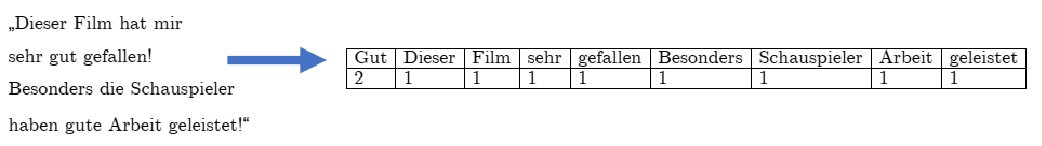
\includegraphics[scale=0.9] {Vect}
\caption[Vektorisierung und Entfernung von Stoppwörtern]{Vektorisierung und Entfernung von Stoppwörtern}
\label{Vect}
\end{figure}

Abbildung \ref{Vect} zeigt, wie einer der Sätze nach Zerlegung des Satzes durch Tokenisierung und Entfernung von Stoppwörtern aussehen könnte. Für mehrere Sätze bzw. Dokumente erweitert sich dieser Vektor zu einer mehrdimensionalen Matrix. Die Spalten stellen dabei alle in der Dokumentensammlung vorkommenden Wörter dar, die Zeilen die einzelnen Dokumente. 

\subsubsection{Wortverarbeitung}
Ein weiterer essentieller Schritt ist die Rückführung der einzelnen Wörter auf ihren Wortstamm, da sonst unterschiedlich konjungierte Wörter vom Algorithmus auch als unterschiedliche Wörter behandelt werden würden, obwohl es sich um das gleiche Wort mit derselben Bedeutung handelt. So würde Beispielsweise das Wort „Trading“ und das Wort „Trade“ ohne vorherige Anpassungen auch als unterschiedliche Worte erkannt und behandelt werden. Ziel der Algorithmen ist es, das jeweilige Wort auf ihren Wortstamm, im Beispiel also „Trade“, zu reduzieren. 

Um dieses Ziel zu erreichen wurden einige Algorithmen entwickelt. Im folgenden Abschnitt werden diese Algorithmen beschrieben und deren Anwendungsweise, Vor- und Nachteile erklärt. 

\paragraph{Porter-Stemmer-Algorithmus}
Ein sehr einfacher, aber effizienter Algorithmus ist der von M.F. Porter (1980) entwickelte Porter-Stemmer-Algorithmus. Der Algorithmus unterscheidet zwischen Konsonanten (im Weiteren c, gemeint sind alle Buchstaben außer A, E, I, O, U, und Y, wenn ein Konsonant vorrausgeht) und Vokalen (v). Eine Folge aus Konsonanten wird als C und eine Folge aus Vokalen als V bezeichnet, wenn diese Folge größer als 0 ist. Alle Wörter können also durch 

\begin{equation}
[C]VCVC...[V]
\end{equation}

oder vereinfacht 

\begin{equation}
[C] (VC)^m [V]
\end{equation}

dargestellt werden, wobei m ein Maß für die Anzahl der Vokal-Konsonant-Kombinationen des Wortes ist. Auf die Wörter werden Regeln der Form 

\begin{equation}
[C] (Bedingung B)S1->S2 [V]
\end{equation}

angewendet, wenn das Wort mit S1 endet, und der Wortteil vor S1 die Bedingung B erfüllt. Insgesamt werden sechs Regeln auf Wörter angewendet. 

\begin{description}

\item[Regel 1:] Reduzierung von Wörtern im Plural und Partizipien.
\item[Regel 2:] Reduzierung von Sonderfällen mit m > 0, z.B.: 

Ational -> Ate

relational -> relate

\item[Regel 3:] Reduzierung von Sonderfällen mit m > 0, z.B.: 

ative ->

formative -> form

\item[Regel 4:] Reduzierung weiterer Sonderfälle mit m > 1, z.B.:

Ance ->

allowance -> allow

\item[Regel 5:] “Aufräumen” bei bestimmten Worten, z.B.:

(m > 1) E ->

probate -> probat

\end{description}

Dieser Algorithmus ist in der Lage, mit geringer Rechenkapazität und geringem Zeitaufwand gute Ergebnisse zu erzielen. 

\paragraph{Lemmatisierung}
Im Unterschied zum Stemming-Algorithmus von M.F. Porter beschränkt sich die Lemmatisierung auf das Kürzen der Wörter durch ein Wörterbuch. Dies hat den Vorteil, dass bei der Umstellung auf eine andere Sprache der Algorithmus nicht angepasst, sondern nur das verwendete Wörterbuch ausgetauscht werden muss. Statt heuristisch die Wörter auf ihren Wortstamm zurückzuführen, wird bei der Lemmatisierung in dem Wörterbuch nach dem entsprechenden Wort gesucht, und dieses dann anhand der Ergebnisse zurückgeführt. \footnote{Vgl. Plisson u.a. (2004), S. 1)} Dies ist im Grunde nicht so fehleranfällig wie Stemming, allerdings werden Wörter die falsch geschrieben sind nicht so einfach erkannt. 

Durch die heuristische Herangehensweise des Stemming-Algorithmus können dort in vielen Fällen aber auch Wörter mit Schreibfehlern erkannt werden. 

Die einfache, wörterbuchbasierte Lemmatisierung wurde durch verschiedene Wissenschaftler um regelbasierte Algorithmen\footnote{z.B. Müller u.a. (2015)} erweitert, die zu einer immer höheren Präzision führen. 


\subsubsection{Vektorisierung}

Da Algorithmen nur mit Zahlen, aber nicht mit Text an sich umgehen können, werden die Texte zunächst in Vektoren zerlegt, welche die Häufigkeit der einzelnen Wörter beschreiben. Im Bereich des maschinellen Lernens werden dafür vor allem zwei Verfahren eingesetzt: das etwas simplere Bag-of-Words-Modell, und das Tf-idf-Maß. Für beide Verfahren werden die Texte zunächst durch Tokenisierung in einzelne Wörter zerlegt. Außerdem wird angenommen, dass der Kontext nur eine untergeordnete Rolle für die Klassifizierung spielt, da die Wörter ungeachtet ihrer Reihenfolge und ihres Zusammenhangs den Vektoren zugeteilt werden, es wird also nur durch die Häufigkeit eines Wortes in einem Text klassifiziert. Die Häufigkeit eines Wortes $w$ in einem Text $d$ wird auch als Term Frequency $TF(w, d)$ bezeichnet. 

Das \textbf{Bag-of-Words-Verfahren}\footnote{Vgl. T. Joachims (2002), S. 13-19}
 verfolgt den Ansatz, dass die Häufigkeit eines Wortes in einem Text Aufschluss über dessen Wichtigkeit zur Klassifizierung gibt. An dieser Stelle wird auch klar, warum es wichtig ist vor der Vektorisierung die Stoppwörter zu entfernen. Da Wörter wie ``I'', ``This'' oder ``and'' keinen großen inhaltlichen Nutzen aufweisen, sollten diese nicht in die Vektorisierung einbezogen werden. 

Das \textbf{Tf-Idf-Maß}\footnote{Vgl. W. Zhang u.a. (2010), S. 2760}
 gewichtet die Wörter in einem Dokument, die häufig vorkommen, geringer als der Bag-of-Words-Ansatz. Tf steht dabei für Term Frequency, also die Vorkommenshäufigkeit und idf für Inverse Document Frequency, die inverse Dokumentenhäufigkeit. Dies hat den Hintergrund, dass die Häufigkeit eines Wortes allein kein gutes Maß für die Wichtigkeit dieses Wortes ist. Besonders bei speziellen Texten, die einem bestimmten Themenkomplex zugeordnet werden können, scheint dies sinnvoll zu sein. So kommen Beispielsweise in Dokumenten über Banken die Wörter ``Bank'' oder ``Trade'' signifikant häufiger vor, ohne dass sich durch diese eine nutzenstiftende Klassifizierung (außer zu dem besagten Themenkomplex, in diesem Fall ``Banking'') ableiten lassen könnte. 

Aus diesem Grund werden Wörter, die mit dem Tf-idf-Maß klassifiziert werden und häufig vorkommen geringer gewichtet. Dies geschieht, indem die Wortgewichtungen durch

\begin{equation}
w_{i,j}=tf_{i,j}*log(\frac{N}{df_i})
\end{equation}

berechnet werden. $w_{i,j}$ repräsentiert die Gewichtung des Wortes $i$ in Dokument $j$, $N$ ist die Anzahl der Dokumente (in unserem späteren Anwendungsfall die Anzahl der Bewertungen), $tf_{i,j}$ die Häufigkeit des Wortes $i$ in Dokument $j$ und $dj_i$ die Anzahl der Dokumente, die das Wort $i$ enthalten. Das Tf-idf-Maß gibt also die Relevanz eines Wortes innerhalb des Dokumentes an. 







\subsection{Algorithmen}
Algorithmen zum maschinellen Lernen existierten schon lange bevor diese nach unserem heutigen Verständnis angewendet wurden. Die Verfügbare Rechnerkapazität war zur Zeit der Entwicklung noch nicht in der Lage, so große Datensätze wie heute üblich zu verarbeiten und die Modelle adäquat zu trainieren. 

Grundsätzlich lassen sich alle Machine-Learning-Algorithmen in zwei Gruppen einteilen: Solche mit überwachtem und solche mit unüberwachtem Lernen. \footnote{Vgl. Z. Ghahramani (2004), S. 3}

Beim überwachten Lernen findet im Vorfeld eine Klassifizierung der Daten (den Eingangsdaten werden erwünschte Ausgangsdaten zugeordnet) statt, durch welche der Algorithmus Muster erkennt und im Anschluss auch Daten zuordnen kann, die nicht Teil des Lernprozesses waren. 

Beim unüberwachten Lernen hingegen werden keine Ausgangsdaten als gewünschte Ergebnisse verarbeitet. Der Algorithmus klassifiziert vielmehr selbst, und versucht durch die erkannten Muster eigene Klassen („Features“) zu erstellen. 



\subsubsection{Lineare Regressionsmodelle, logistische Regression}
Als einfachster Machine-Learning-Algorithmus wird oft die lineare Regression (für Regressionsaufgaben) bzw. die logistische Regression (Klassifizierungsprobleme) angeführt. Dieser Algorithmus entstammt der Statistik und wird dort bereits lange verwendet, hat aber auch auf bestimmten Gebieten des Machine Learning Anwendung zur Prognose und Klassifizierung gefunden. Ursprünglich wurde die lineare Regression zur Voraussage bestimmter zukünftiger Zustände auf Basis von heute bekannten Daten verwendet. 

Das lineare Regressionsmodell erlaubt es, eine abhängige Variable $y$ durch eine unabhängige Variable $x$ zu beschreiben. \footnote{Vgl. Wooldridge (2008)}
Das einfache lineare Regressionsmodell lässt sich durch

\begin{equation}
y=\beta_0+\beta_1 x+\mu
\end{equation}

beschreiben. $\beta_0$ ist der y-Achsenabschnitt, während $\beta_1$ den Einfluss der Variable $x$ ceteris paribus auf y darstellt. Der Parameter $\mu$ beschreibt alle Faktoren, die nicht durch $x$ beschrieben werden können, aber trotzdem einen Einfluss auf den Wert von $y$ haben. $\mu$ wird deswegen auch als Fehlerterm bezeichnet. 
$\beta_1$ wird durch kleinste-Quadrate-Schätzung 

\begin{equation}
\hat{\beta}_1=\frac{\sum_{i=1}^n(x_i-\bar{x})(y_i-\bar{y} )}{\sum_{i=1}^n (x_i-\bar{x})^2 }
\end{equation}

bestimmt. Der obere Teil des Bruchs entspricht der Kovarianz der Stichprobe zwischen $x$ und $y$, während der untere Teil die Varianz von $x$ ist. 
$\beta_0$ lässt sich im Anschluss einfach berechnen durch 

\begin{equation}
\beta_0=\bar{y}-\hat{\beta}_1 \bar{x}
\end{equation}

wobei $\bar(y)$ das arithmetische Mittel der abhängigen und $\bar(x)$ der unabhängigen Variable ist.
Zusammensetzten der Parameter ergibt dann: 

\begin{equation}
\hat{y}=\hat{\beta}_0+\hat{\beta}_1 x.
\end{equation}

$\hat{y} $ kennzeichnet, dass die Parameter aus der Probe geschätzt wurden (sie werden auch als Schätzer bezeichnet). 

Im Gegensatz zum linearen Regressionsmodell verwendet die logistische Regression als Verteilungsannahme die kumulierte logistische Wahrscheinlichkeitsfunktion $F$. Außerdem handelt es sich bei der logistischen Regression im Gegensatz zum linearen Regressionsmodell um einen Klassifizierungsalgorithmus. Das Ergebnis der logistischen Regression wird durch die Funktion $F$ in einen Wertebereich zwischen 0 und 1 gebracht, was dann eine Klassifizierung ermöglicht. 

\begin{equation}
Pr(Y=1|X_1)=F(\beta_0+\beta_1X_1)
= \frac{1}{1+e^{-(\beta_0+\beta_1X_1)}}
\end{equation}

Die Funktion gibt als Ergebnis die Wahrscheinlichkeit an, dass die unabhängige Variable $X_1$ den Wert 1 annimmt. \footnote{Vgl. J. Stock, M. Watson (2012) S. 394}

\subsubsection{Stochastic Gradient Descent}

Für große Datensätze geeignet sind Gradient Descent (``Gradientenabstieg'')-Algorithmen. Das Verfahren verfolgt dabei einen iterativen Ansatz, nähert sich der Lösung also schrittweise, bis zur Überschreitung eines Toleranzterms, an. Gradient Descent-Algorithmen passen einen Gewichtungsparameter $w$ durch die Funktion

\begin{equation}
w_{t+1}=w_t-\gamma\frac{1}{n}\sum_{i=1}^n\nabla_wQ(z_i, w_t)
\end{equation}

an. $\gamma$ entspricht dabei der Schrittgröße, also der Rate, mit dem der Algorithmus den Gewichtungsparameter anpasst. Dieser Parameter wird auch als Lernrate bezeichnet. 

Eine Vereinfachung des Gradient Descent-Verfahrens ist der Stochastic Gradient Descent-Algorithmus (``Stochastischer Gradientenabstieg'') \footnote{Vgl. L. Bottou (2012)}.

\begin{equation}
w_{t+1}=w_t-\lambda_t\nabla_wQ(z_t,w_t)
\end{equation}

Dabei wird der Gradient nicht exakt berechnet, sondern in jedem Iterationsschritt zufällig durch Randomisierung des Parameters $z_t$ geschätzt. 


\subsubsection{Naive Bayes Classifier}

Ein ebenfalls weit vor der Verbreitung von Maschinellem Lernen nach dem heutigen Verständnis entworfener Algorithmus ist der Naive Bayes Classifier, welcher auf dem aus der Statistik bekanntem Bayes-Theorem aufbaut. Naive Bayes Classifier werden trotz ihrer langsamen Performance weiterhin sehr häufig zur Textklassifizierung genutzt, da sie schnell und einfach zu implementieren sind. \footnote{Vgl. Rennie u.a. (2003), S. 1}

Da der Kern dieser Arbeit sich mit der Textklassifizierung befasst, wird im Folgenden das für dieses Gebiet geeignete Modell des multinominalen Naive Bayes erklärt. Das multinominale Modell eignet sich besser, da es die Wahrscheinlichkeit vieler Ereignisse, in unserem Fall das Auftreten von Wörtern in einem Text, auf einmal betrachtet. 

Ein Text wird bei diesem Algorithmus als Sequenz von Wörtern betrachtet. Klassifizierung findet über verschiedene Klassen statt, wobei jeder Klasse $(c \in{1,2,…m})$ ein Parametervektor der Form $\vec{\theta}_c={\theta_{c1},\theta_{c2},…,\theta_{cn}}$ zugeordnet wird. n entspricht der Größe des Vokabulars, also der Anzahl der unterschiedlichen Wörter im Text. $\theta_{ci}$ entspricht der Häufigkeit des Wortes innerhalb der Klasse. 

Durch die Funktion 

\begin{equation}
\hat{\theta}_{ci}=\frac{N_{ci}+\alpha_i}{N_c+\alpha}
\end{equation}

wird der Häufigkeitsparameter für Wort i der Klasse c bestimmt., $N_{ci}$ ist die Häufigkeit des Wortes i in Klasse c, $N_c$ die Summe aller Wörter in Klasse c, $\alpha_i$ ein Glättungsparameter und $\alpha$ die Summe dieser Parameter. Zur Vereinfachung kann der Glättungsparameter in den meisten Fällen auf eins gesetzt werden. 
Die Klassifizierungsfunktion mit der höchsten summierten Wahrscheinlichkeit (Likelihood) berechnet sich abschließend durch 

\begin{equation}
l_{MNB}(d)=argmax_c \left[log\hat{p}(\theta_c)+\sum_i{f_i log\frac{N_{ci}+\alpha_i}{N_c+\alpha}}\right]
\end{equation}

Diese Funktion wird nun zur Klassifizierung genutzt.


\subsubsection{Random Forests}

Random Forest-Algorithmen klassifizieren durch die zufällige Erstellung von unkorrelierten Entscheidungsbäumen. Entscheidungsbäume sind bei Randon Forest-Algorithmen zufällig, da die Faktoren, nach denen die Daten an den Knoten unterteilt werden, zufällig aus der Gesamtheit der zur Verfügung stehenden Faktoren gewählt werden. Dies sorgt auch dafür, dass die Entscheidungsbäume nicht mehr korreliert sind. Dadurch kommt es zu einer Diversifikation bei der Faktorenauswahl, was schlussendlich zu einer hohen Voraussagekraft des Algorithmus führt.\footnote{Vgl. T. Yiu} Genauer wird für jeden Baum ein zufälliger Vektor erstellt, welcher unabhängig von den vorangegangenen Vektoren ist, allerdings dieselbe Wahrscheinlichkeitsverteilung besitzt. Aus dem Trainings-Datensatz und dem zufälligen Vektor ($\Theta_k$) wird im Anschluss die Klassifizierungsfunktion 

\begin{equation}
h(x,\Theta_k)
\end{equation}

gebildet. $x$ entspricht hier dem Input-Vektor. Wenn eine Vielzahl an Bäumen generiert wurde, findet der Klassifizierungsprozess statt. Jeder Baum darf in diesem Prozess eine Entscheidung für eine bestimmte Klasse treffen. Die Klasse mit den meisten Stimmen wird dann für die endgültige Klassifizierung genutzt. \footnote{Vgl. Breiman (2001), S. 2}

Zur Generierung der Entscheidungsbäume stehen unterschiedliche Algorithmen zur Verfügung. Beim „bagging“ werden aus der Grundgesamtheit zufällig Trainingsdatensätze mit zufälligen Parametern gezogen. Aus diesem Datensatz wird im Anschluss ein Entscheidungsbaum generiert. \footnote{Vgl. Breiman (2001), S. 8}

Ein weiterer, darauf aufbauender Algorithmus ist AdaBoost. Bei diesem Algorithmus wird aus einer Vielzahl “schwacher” Klassifikatoren (sie berücksichtigen nur wenige Merkmale der betrachteten Objekte) ein starker Klassifikator generiert, indem die schwachen Klassifikatoren, welche die besten Ergebnisse erzielen, höher gewichtet werden. \footnote{Vgl. Y. Freund, R. Schapire (1996)}

\subsubsection{Mehrlagiges Perzeptron (MLP, Multi-Layer Perceptron)}


Das von Psychologe Rosenblatt (1958) entwickelte Modell der mehrlagigen Perzeptronen gilt als eines der ersten und einfachsten künstlichen neuronalen Netzwerke. 
Ein künstliches mehrlagiges Perzeptron besteht aus mehreren Knoten, die durch gewichtete Zweige miteinander verbunden sind. Diese Zweige lassen sich mit aus der Neurobiologie bekannten Synapsen vergleichen. Die Mehrlagigkeit zeichnet sich dadurch aus, dass es mehrere Schichten von künstlichen Neuronen gibt. Unterschieden wird zwischen drei Arten von Schichten: Die Eingabeschicht (Input Layer), die Zwischenschichten (Hidden Layer) und die Ausgabeschicht (Output Layer). 

Die Eingabeschicht ist immer mit einer oder mehreren Zwischenschichten verbunden. Sie verteilt die Eingangsvariablen auf die Knoten der Zwischenschichten. 
Ein neuronales Netzwerk kann weiterhin aus einer oder mehreren Zwischenschichten bestehen, welche wiederrum aus mehreren Knoten bestehen. Die letzte Zwischenschicht gibt die Ergebnisse an die Ausgabeschicht weiter. Die Ausgabeschicht normalisiert das Ergebnis im Anschluss noch auf einen vordefinierten Wertebereich. 

Abbildung \ref{mlp} zeigt beispielhaft den Aufbau eines mehrlagigen Perzeptrons mit einer Zwischenschicht und drei Knoten auf dieser Zwischenschicht. 


\begin{figure}[ht]
\centering
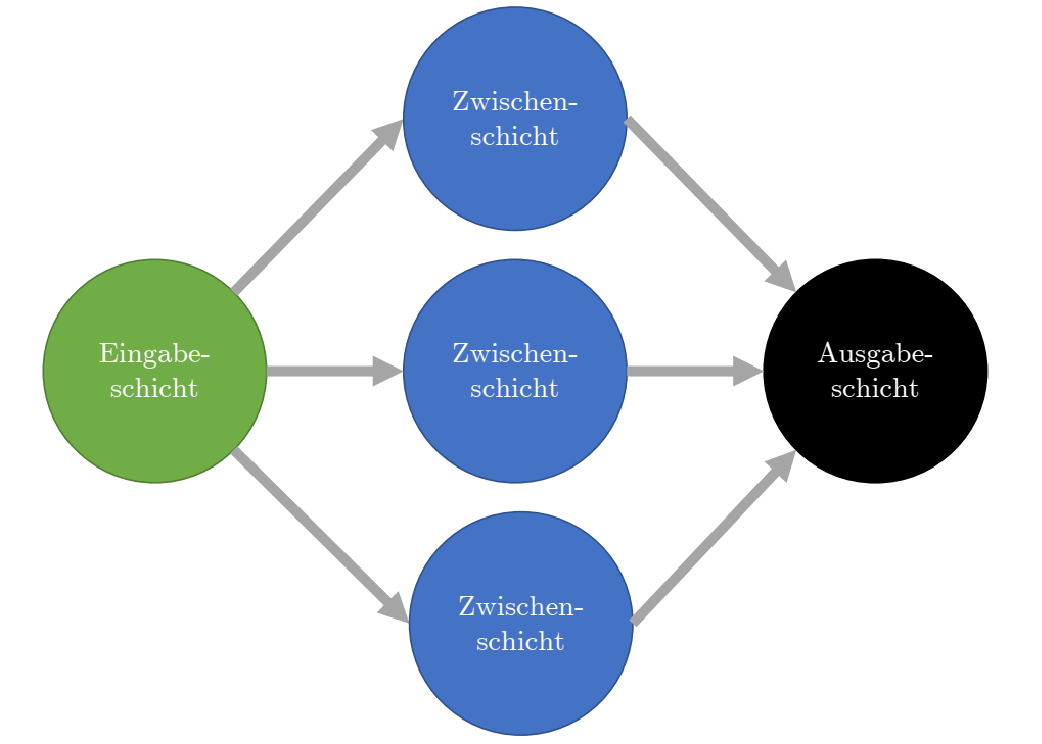
\includegraphics[scale=0.7] {mlp}
\caption[Beispielhafte Abbildung eines mehrlagigen Perzeptrons mit einer Zwischenschicht]{Beispielhafte Abbildung eines mehrlagigen Perzeptrons mit einer Zwischenschicht}
\label{mlp}
\end{figure}

Die Ausgabeschicht ist immer mit der letzten Zwischenschicht verbunden. Innerhalb der Schichten bestehen keine Verbindungen zwischen den Knoten. 
Um das neuronale Netzwerk nun anzulernen, werden die Gewichtungen an den Knoten zuerst zufällig gesetzt. Im Anschluss wird Vektor für Vektor der Trainingsdatensatz durch die Eingabeschicht eingelesen. Anschließend wird der Ausgabewert des Netzwerkes mit dem Wert verglichen, welcher nach dem Trainingsdatensatz zu erwarten wäre. Die Gewichtungen werden dann so angepasst, dass das Ergebnis näher an dem des Trainingsdatensatzes liegt. Dieser Vorgang wird iterativ mit allen Eingabevektoren des Trainingsdatensatzes durchgeführt. 
Dieser Trainingsvorgang kann beispielsweise durch Fehlerrückführung realisiert werden. In einem ersten Schritt sind die Parameter des Netzwerkes konstant. Ein erstes Eingangssignal durchläuft das Netzwerk. Abschließend wird ein Fehlerwert durch 

\begin{equation}
e_i=d_i-y_i
\end{equation}

berechnet, wobei $d_i$ das gewünschte Ergebnis und $y_i$ das durch das Netzwerk realisierte Ergebnis ist. Dieser Fehlerterm durchläuft das Netzwerk nun in umgekehrter Reihenfolge, wobei die Parameter so angepasst werden, dass sie den Fehlerterm minimieren. \footnote{Vgl. M. Ettaouil u.a. (2013)}


\subsubsection{Bird-Swarm-Algorithmus}

Ein weiterer von der Natur inspirierter Algorithmus ist der Bird-Swarm-Algorithmus. \footnote{Meng u.a. (2015)} Dieser Algorithmus basiert auf dem Herdenverhalten von Vogelschwärmen. Der Algorithmus kann durch fünf Regeln abstrahiert werden:

\begin{description}

\item[Regel 1:] Die Vögel können in einem von zwei Zuständen sein: Wachsamkeit oder Futtersuche.

\item[Regel 2:] Während der Futtersuche erinnert sich jeder Vogel an die beste Futterposition.

\item[Regel 3:] Während der Wachsamkeit versucht jeder Vogel in die Mitte des Schwarms zu kommen. 

\item[Regel 4:] Vögel bewegen sich innerhalb des Schwarms. Vögel mit hohen Futterreserven sind Futtersammler, Vögel mit geringen Reserven Futterdiebe.

\item[Regel 5:] Futtersammler leiten die Futtersuche, während Futterdiebe diesen Sammlern zufällig folgen. 

\end{description}

Um den Algorithmus bei maschinellem Lernen anzuwenden, werden die einzelnen Vögel als Gewichtungen der Knoten eines neuronalen Netzwerkes verwendet. Die Gewichtungen werden wie folgt berechnet:

Im ersten Schritt werden $N$ Vögel zufällig in einem $D$-Dimensionalen Suchraum generiert. Regel zwei errechnet sich durch 

\begin{equation}
x_{i,j}^{t+1}=x_{i,j}^t+(p_{i,j}-x_{i,j}^t)*C *rand_a+(g_j-x_{i,j}^t)*S*rand_a
\end{equation}

wobei $x_{i,j}^t$ der Wert des Elements $j$ von Vogel $i$ in der Generation $t$ mit $i \in [1,...,N]$ und $j \in [1,...,D]$ ist. $rand_a$ sei ein Zufallswert zwischen 0 und 1. $C$ und $S$ seien ein kognitiver und ein sozialer Koeffizient, repräsentieren also das Verhalten innerhalb des Schwarms und die Interaktionen der Vögel. $P_{i,j}$ und $g_i$ sei die persönliche und globale (also die des Schwarms) Erfahrung. 

Der Anfangszustand eines Vogels (Regel 1) wird zufällig generiert. Die Bewegung der Vögel zur Mitte des Schwarms (Regel 3) wird durch

\begin{equation}
x_{i,j}^{t+1}=x_{i,j}^t+A'1(mean_j-x_{i,j}^t)*C *rand_a+A2(p_{k,j}-x_{i,j}^t)*S*rand_b
\end{equation}

\begin{equation}
A1=a1*exp\left(\frac{pFit_i}{sumFit+\epsilon}*N\right)
\end{equation}

\begin{equation}
A2=a2*exp\left(\left(\frac{pFit_i-pFit_k}{|pFit_k-pFit_i|+\epsilon}\right)\frac{N*pFit_k}{sumFit+\epsilon}\right)
\end{equation}

berechnet. $a1$ und $a2$ seien positive Konstanten zwischen 0 und 2. $pFit_i$ ist der optimiert Wert des Vogels $i$, $sumFit$ die Summe aller dieser Werte, $\epsilon$ eine sehr kleine Konstante, um Dividieren durch 0 zu vermeiden, $mean_j$ sei der Wert des $j$en Elements der durchschnittlichen Position alles Vögel im Schwarm. 

Abschließend werden die Futtersammler durch 

\begin{equation}
x_{i,j}^{t+1}=x_{i,j}^t+randn*x_{i,j}^t
\end{equation}

und 

\begin{equation}
x_{i,k}^{t+1}=x_{i,j}^t+(x_{k,j}^t-x_{i,j}^t)*FL*rand_a
\end{equation}

modelliert. $randn$ entspricht einem zufälligem, gaußverteiltem Wert mit Mittelwert 0 und Standardabweichung 1, $k \in [1,...,N]$, $k\neq i$ und $FL \in [0,2]$.


\section{Anwendung}

Um die vorhergehend erläuterten Prozesse und Algorithmen anzuwenden, verwenden wir Datensätze von drei verschiedenen Bewertungsportalen: imdb.com (Filme), amazon.com (Verbrauchsgüter) und yelp.com (Lokalitäten). \footnote{J. Rennie u.a. (2015)} Die Datensätze sind bereits mit einem Stimmungsindikator versehen, welcher entweder auf 1 (positive Bewertung) oder auf 0 (negative Bewertung) gesetzt wurde. Dieser Parameter ist wichtig, um den Algorithmen das Erlenen einer Klassifizierung zu ermöglichen. Für jede Internetseite besteht der Datensatz jeweils aus 500 positiven und 500 negativen Bewertungen, wobei keine neutralen Bewertungen einbezogen wurden. 

Um den Unterschied zwischen dem Bad-of-Words- und dem Tf-idf-Verfahren zu analysieren, wurden die Datensätze mit jeweils beiden Verfahren in unterschiedlichen Vorgängen Vektorisiert. 

\begin{table}[h]
\centering
\begin{tabular}{|ll|ll|ll|}
\hline
\multicolumn{2}{|c|}{\textbf{Amazon}}&\multicolumn{2}{c}{\textbf{Yelp}}&\multicolumn{2}{|c|}{\textbf{Imdb}} \\
\hline
\textbf{Wort} & \textbf{Häufigkeit} & \textbf{Wort} & \textbf{Häufigkeit} &\textbf{Wort} & \textbf{Häufigkeit} \\
\hline
phone & 126 & food & 93 & movie & 134 \\
great & 77 & place & 78 & film & 113 \\
good & 54 & good & 72 & just & 45 \\
product & 46 & service & 58 & bad & 43 \\
headset & 41 & great & 53 & good & 41 \\
quality & 40 & like & 37 & time & 34 \\
sound & 35 & time & 33 & like & 34 \\
battery & 32 & just & 30 & great & 32 \\
works & 32 & really & 27 & really & 31 \\
use& 30 & best & 25 & characters & 29 \\
\hline
\end{tabular}
\caption{Worthäufigkeit Bag-of-Words}
\label{BoW}
\end{table}

In Tabelle \ref{BoW} sind die absoluten Worthäufigkeiten des Bag-of-Words-Verfahrens angegeben. Es ist ersichtlich, dass bis auf den Imdb-Datensatz die positiven Begriffe (vor allem ``great'' und ``good'') überwiegen, während der Imdb-Datensatz verhältnismäßig mehr negative Begriffe (``bad'') aufweist. Außerdem scheinen die meisten Bewertungen des Amazon-Datensatzes über Mobiltelefone zu sein, während der Yelp-Datensatz vor allem Restaurantkritiken enthält. 

Allerdings zeigt sich auch, dass zur Klassifizierung Wörter verwendet werden, aus denen sich nur schwer eine Aussage über die Meinung des Schreibers ableiten lässt. Dies sind vor allem Wörter, die sich auf das bewertete Produkt bzw. die Dienstleistung beziehen (im speziellen: ``phone'', ``headset'', ``food'', ``place'', ``movie'', ``film'').

\begin{table}[h]
\centering
\begin{tabular}{|ll|ll|ll|}
\hline
\multicolumn{2}{|c|}{\textbf{Amazon}}&\multicolumn{2}{c}{\textbf{Yelp}}&\multicolumn{2}{|c|}{\textbf{Imdb}} \\
\hline
\textbf{Wort} & \textbf{Häufigkeit} & \textbf{Wort} & \textbf{Häufigkeit} &\textbf{Wort} & \textbf{Häufigkeit} \\
\hline
phone & 30,71 & food & 25,28 & movie & 22,36 \\
great & 29,95 & good & 24,63 & film & 19,52 \\
good & 20,3 & place & 24,05 & bad & 12,15 \\
product & 18,75 & service & 20,74 & just & 10,58 \\
works & 14,48 & great & 17,2 & good & 9,94 \\
quality & 13,58 & time & 11,26 & 10 & 9,75 \\
headset & 12,71 & like & 10,7 & great & 8,4 \\
price & 12,2 & won & 9,71 & really & 7,57 \\
sound & 11,27 & just & 9,38 & time & 7,45 \\
recommed & 11,16 & really & 9 & acting & 6,67 \\
\hline
\end{tabular}
\caption{Worthäufigkeit Tf-idf}
\label{Tfidf}
\end{table}

Tabelle \ref{Tfidf} zeigt die Worthäufigkeiten nach Vektorisierung durch das Tf-idf-Verfahren. Wörter, die sich besser zur Klassifizierung eignen (vor allem ``works'' [Amazon], ``good'' [Yelp] und ``bad'' [Imdb]), werden höher gewichtet als es nach dem Bag-of-Words-Verfahren der Fall ist. Daraus lässt sich der Schluss ziehen, dass sich das Tf-idf-Verfahren für unseren Anwendungsfall besser eignet, da so eine präzisere Klassifizierung möglich ist.

Die Datensätze werden vor der Vektorisierung noch in einen Trainings- und einen Testdatensatz aufgeteilt. Dies geschieht über die zufällige Auswahl einer gewissen Anzahl an Datenpunkten aus dem gesamten Datensatz. Die Größe des Test-Datensatzes beträgt in unserem Fall 35\%, während der Trainings-Datensatz 65\% der Daten enthält.

Nach Vektorisierung der einzelnen Bewertungen werden im Folgenden die Machine-Learning-Algorithmen auf den Datensatz angewandt. Auf Anwendung des Bird-Swarm-Algorithmus wurde hier verzichtet, da der Algorithmus noch sehr neu ist und es aktuell keine einfach zu implementierenden Python-Pakete für diesen Algorithmus gibt.

Nach mehreren Testdurchläufen wurden die folgenden Parameter als am effizientesten identifiziert:

\begin{description}

\item{\textbf{Logistic Regression:}} \\
Verwendung der Standardparameter

\item{\textbf{Stochastic Gradient Descent:}} \\
loss: ``squared\_hinge'' - quadrierte Form der normalen Verlustfunktion \\
alpha: 0.0001 - Konstante, mit welcher der Regularisierungswert multipliziert wird \\
tol: 0.00001 - Stoppkriterium \\
random\_state: 0 - Startwert für die Generierung der zufälligen Werte \\
eta0: 0.0001 - Startlernrate

\item{\textbf{Random Forest:}} \\
n\_estimators: 1000 - Anzahl der Bäume \\
random\_state: 0 - Startwert für die Generierung der zufälligen Werte 

\item{\textbf{Support Vector Machine:}} \\
Verwendung der Standardparameter

\item{\textbf{Multi Layer Perceptron}} \\
solver: `adam' - Stochastic Gradient-Optimierungsfunktion \\
alpha: 0.00001 - Konstante, mit welcher der Regularisierungswert multipliziert wird \\
hidden\_layer\_sizes: (4, 12) - Anzahl der Zwischenschichten, Anzahl der Neuronen pro Zwischenschicht \\
max\_iter: 1000 - maximale Anzahl an Iterationen \\
random\_state: 0 - Startwert für die Generierung der zufälligen Werte


\end{description}


Nach Training der Algorithmen und Auswertung mit Hilfe der Testdatensätze wurden die in Tabelle \ref{accuracy} gezeigten Genauigkeiten erzielt. Der Wert gibt an, wie viele der Test-Daten korrekt klassifiziert wurden. 


\begin{table}[h]
\centering
\begin{tabular}{|l|lll|}
\hline
\textbf{Algorithmus} & \textbf{Amazon} & \textbf{Yelp} & \textbf{Imdb} \\
\hline
Logistic Regression & 0,7950 & 0,7750 & 0,7633 \\
Stochastic Gradien Descent & 0,7075 & 0,7175 & 0,6567 \\
Random Forest & 0,7625 & 0,7525 & 0,6767 \\
Support Vector Machine & 0,8000 & 0,7700 & 0,7467 \\
Multi Layer Perceptron & 0,7450 & 0,7325 & 0,7333 \\

\hline
\end{tabular}
\caption{Genauigkeit der Algorithmen}
\label{accuracy}
\end{table}

Es zeigt sich, dass vor allem die Logistische Regression und die Support Vector Machine die besten Ergebnisse über alle Datensätze hinweg erzielten. Außerdem scheint die Klassifizierung des Amazon-Datensatzes am besten zu funktionieren, während die Genauigkeiten des Yelp- und des Imdb-Datensatzes leicht darunter liegen. Dies hängt vermutlich mit dem im Text verwendeten Begriffen zusammen, der Amazon-Datensatz scheint also über mehr Wörter zu verfügen, die eine genaue Klassifizierung ermöglichen. 

Dies wird auch durch die oben bereits dargelegte Darstellung der Worthäufigkeiten deutlich. Im Amazon-Datensatz sind häufiger Wörter enthalten, aus welchen sich eine Wertung ableiten lässt. 

Weitere Werte, die Aufschluss über die Effizienz des verwendeten Algorithmus geben, ist unter anderem die zum Training des Modells verwendete Zeit. Dieser Parameter ist besonders wichtig für große Datensätze, da eine geringere Zeit zum Training eine schnellere Verwendung des Modells ermöglicht. 

Die besten Ergebnisse erzielte hier der Stochastic Gradient Descent-Algorithmus mit einer Trainingszeit von rund 0,001 Sekunden bei allen Datensätzen. Mit Abstand die meiste Zeit brauchte der Random Forest-Algorithmus. Er benötigte im Schnitt drei Sekunden, um das Modell anzulernen. 

Die bei der Genauigkeit am besten abgeschnittene logistische Regression benötigte Durchschnittlich 0,001 Sekunden. Auch der Support-Vector-Machine-Algorithmus benötigte mit einer Trainingszeit von circa 0,02 Sekunden nicht viel mehr Zeit als die anderen Algorithmen, bei gleichzeitig guter Genauigkeit.

Aus den oben angeführt Parametern wird klar, dass die logistische Regression und die Support Vector Machine sowohl bei der Genauigkeit als auch bei der verwendeten Trainingszeit die besten Ergebnisse erzielen. Daraus lässt sich der Schluss ziehen, dass diese beiden Algorithmen sich für die Klassifizierung der von uns verwendeten Datensätze am besten eignen. 

Allerdings lässt sich dieses Ergebnis nicht auf alle Textdatensätze anwenden. Die in den vorhergehenden Abschnitten erläuterten Verfahren zur Vektorisierung und Auswahl von Algorithmen geben einen Einblick über die Vorarbeit, welche geleistet werden muss, um einen effizienten Algorithmus für die Klassifizierung von Textdaten zu bestimmen. Dieses Verfahren muss auf alle neuen Datensätze angewendet werden, um konsistent präzise Ergebnisse zu erzielen. 


\section{Fazit}
Machine Learning wird auch weiter eine äußerst wichtige Teildisziplin bleiben und alle uns bekannten Geschäftsfelder mehr oder weniger beeinflussen. Bis einschließlich 2025 will die Bundesregierung drei Milliarden Euro für die Forschung und Entwicklung im Bereich der künstlichen Intelligenz zur Verfügung stellen. Allerdings wird diese Förderung auch von vielen Seiten, vor allem von Brancheninsidern, als zu gering bewertet. \footnote{Doll u.a. (2018)} Es zeigt sich aber, dass künstliche Intelligenz einen zum heutigen Zeitpunkt noch nicht wirklich quantifizierbaren Einfluss auf unser Leben in allen Bereichen haben wird. 

Diese Arbeit soll einen generellen Überblick über die zur Verfügung stehenden Klassifizierungsalgorithmen und deren spezielle Anwendung im Bereich der natürlichen Sprachverarbeitung geben. Die Analyse der Testdatensätze zeigte, dass sich die logistische Regression und Support Vector-Machine-Algorithmen am besten für die von uns analysierten Datensätze eignen, und eine Vorhersagegenauigkeit von rund 80\% erzielt werden konnte. 
Weitere Arbeiten sollten sich mit der Evaluierung größerer Datensätze und weiterer Algorithmen beschäftigen. Insbesondere der Bird-Swarm-Algorithmus sollte als weiterer Klassifizierungsalgorithmus genauer betrachtet, und in weiteren Arbeiten implementiert werden. 


\newpage
\begin{thebibliography}{9}

\bibitem{Bottou}
Bottou, L. (2012). Stochastic Gradient Descent Tricks. Lecture Notes in Computer Science Neural Networks: Tricks of the Trade, 421–436. doi: 10.1007/978-3-642-35289-8\_25
\bibitem{ Breiman }
Breiman, L. (2001). Machine Learning, 45(3), 261–277. doi: 10.1023/a:1017934522171
\bibitem{ Doll }
Doll, V. N., Doll, N., Fuest, B., Heuzeroth, T., Eckert, D., Schönstein, J., … Boldt, K. (2018, November 14). Künstliche Intelligenz: Deutschland investiert Milliarden in neue Techniken - WELT. Retrieved from https://www.welt.de/wirtschaft/article183877012/Kuenstliche-Intelligenz-Deutschland-investiert-Milliarden-in-neue-Techniken.html
\bibitem{ Ettaouil }

Ettaouil, M., Lazaar, M., \& Ghanuou, Y. (2013). ARCHITECTURE OPTIMIZATION MODEL FOR THE MULTILAYER PERCEPTRON AND CLUSTERING. Journal of Theoretical and Applied Information Technology, 47(1), 64–72.

\bibitem{ Freund }
Freund, Y., \& Schapire, R. E. (1996). Experiments with a New Boosting Algorithm.
Ghahramani, Z. (2004). Unsupervised Learning. Advanced Lectures on Machine Learning Lecture Notes in Computer Science, 72–112. doi: 10.1007/978-3-540-28650-9\_5

\bibitem{ Joachims }
Joachims, T. (2002). Support Vector Machines. Learning to Classify Text Using Support Vector Machines, 35–44. doi: 10.1007/978-1-4615-0907-3\_3

\bibitem{dataset}
Kotzias, D., Denil, M., Freitas, N. D., \& Smyth, P. (2015). From Group to Individual Labels Using Deep Features. Proceedings of the 21th ACM SIGKDD International Conference on Knowledge Discovery and Data Mining - KDD 15. doi: 10.1145/2783258.2783380 

\bibitem{ Meng }
Meng, X.-B., Gao, X., Lu, L., Liu, Y., \& Zhang, H. (2015). A new bio-inspired optimisation algorithm: Bird Swarm Algorithm. Journal of Experimental \& Theoretical Artificial Intelligence, 28(4), 673–687. doi: 10.1080/0952813x.2015.1042530

\bibitem{ Müller }
Müller, T., Cotterell, R., Fraser, A., \& Schütze, H. (2015). Joint Lemmatization and Morphological Tagging with Lemming. Proceedings of the 2015 Conference on Empirical Methods in Natural Language Processing. doi: 10.18653/v1/d15-1272

\bibitem{plisson}
Plisson, J., Lavrac, N., \& Mladenic, D. (2004). A Rule based Approach to Word Lemmatization. Proceedings of IS04. 

\bibitem{ Porter }
Porter, M. (1980). An algorithm for suffix stripping. Program, 14(3), 130–137. doi: 10.1108/eb046814

\bibitem{ Rennie }
Rennie, J. D. M., Shih, L., Teevan, J., \& Karger, D. R. (2003). Tackling the Poor Assumptions of Naive Bayes Text Classi 
ers. Proceedings of the Twentieth International Conference on Machine Learning, (ICML-2003). Retrieved from https://people.csail.mit.edu/jrennie/papers/icml03-nb.pdf

\bibitem{ Rosenblatt }
Rosenblatt, F. (1958). The perceptron: A probabilistic model for information storage and organization in the brain. Psychological Review, 65(6), 386–408. doi: 10.1037/h0042519

\bibitem{ Stock }
Stock, J. H., \& Watson, M. W. (2012). Introduction to econometrics. Boston, MA: Pearson.
Wooldridge, J. M. (2008). Introductory econometrics: a modern approach. Mason, OH: South-Western College Pub.

\bibitem{Zhang}
Zhang, W., Yoshida, T., \& Tang, X. (2011). A comparative study of TF*IDF, LSI and multi-words for text classification. Expert Systems with Applications, 38(3), 2758–2765. doi: 10.1016/j.eswa.2010.08.066

\bibitem{yiu}

Yiu, T. (2019, August 14). Understanding Random Forest. Abgerufen 15. Januar, 2020, \url{https://towardsdatascience.com/understanding-random-forest-58381e0602d2}




\end{thebibliography}





\end{document}


